\begin{pastexam}[label={px:nccu-115-dsa-11}]{政大資科所 115 學年度 第 11 題}
（問答）

Consider the following graph:

\begin{center}
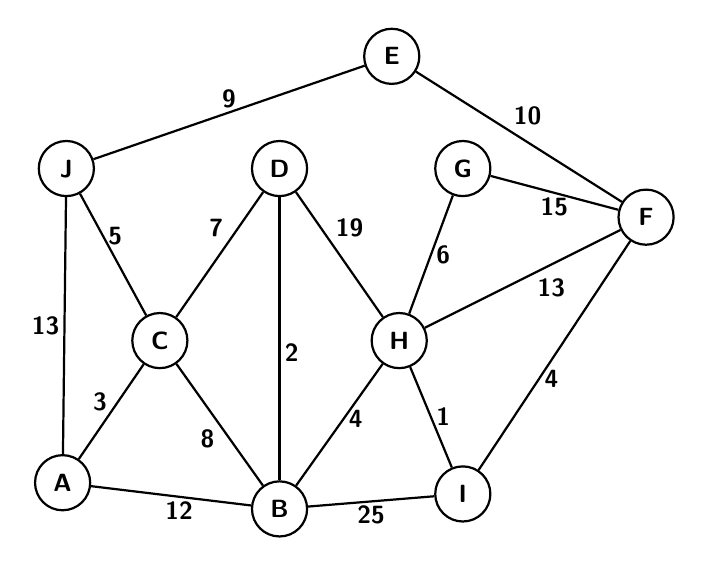
\begin{tikzpicture}[x=0.95cm,y=0.95cm,v/.style={circle,draw,thick,fill=white,inner sep=1pt,minimum size=7mm,font=\small\sffamily\bfseries},
  w/.style={font=\small\sffamily\bfseries,inner sep=1.5pt}]
\node[v] (E) at (5.4,6.05) {E};
\node[v] (J) at (1.05,4.55) {J};
\node[v] (D) at (3.9,4.55) {D};
\node[v] (G) at (6.35,4.55) {G};
\node[v] (F) at (8.8,3.9) {F};
\node[v] (C) at (2.3,2.25) {C};
\node[v] (H) at (5.5,2.25) {H};
\node[v] (A) at (1.0,0.35) {A};
\node[v] (B) at (3.9,0) {B};
\node[v] (I) at (6.35,0.2) {I};
\draw[thick] (J)--node[w,above,pos=0.5]{9}(E);
\draw[thick] (E)--node[w,above right,pos=0.45]{10}(F);
\draw[thick] (G)--node[w,below,pos=0.5]{15}(F);
\draw[thick] (J)--node[w,right,pos=0.35]{5}(C);
\draw[thick] (J)--node[w,left,pos=0.5]{13}(A);
\draw[thick] (D)--node[w,above left,pos=0.4]{7}(C);
\draw[thick] (D)--node[w,right,pos=0.55]{2}(B);
\draw[thick] (D)--node[w,above right,pos=0.4]{19}(H);
\draw[thick] (G)--node[w,right,pos=0.5]{6}(H);
\draw[thick] (H)--node[w,below right,pos=0.55]{13}(F);
\draw[thick] (C)--node[w,left=2pt,pos=0.4]{3}(A);
\draw[thick] (C)--node[w,below left,pos=0.5]{8}(B);
\draw[thick] (H)--node[w,right,pos=0.45]{4}(B);
\draw[thick] (H)--node[w,right,pos=0.5]{1}(I);
\draw[thick] (F)--node[w,right,pos=0.6]{4}(I);
\draw[thick] (A)--node[w,below,pos=0.55]{12}(B);
\draw[thick] (B)--node[w,below,pos=0.5]{25}(I);
\end{tikzpicture}
\end{center}

(a) (5\%) Apply Prim's algorithm, starting from node A, to construct the minimum spanning tree. List the
edges of the minimum spanning tree in the exact order they are added by the algorithm. Use the format
(node1, node2).

(b) (5\%) State the final total weight of the constructed minimum spanning tree.
\end{pastexam}

\begin{pastsoln}
(a) (A, C), (C, J), (C, D), (D, B), (B, H), (H, I), (I, F), (H, G), (J, E)。\quad
(b) $41$。

圖有 $10$ 個點、$17$ 條邊。 Prim（資結書第~24.3~節，虛擬碼~24.3）從 A 開始，每一步在「一端在樹裡、
一端不在樹裡」的邊（跨越切割的邊）中選權重最小的加進來，由資結書定理~24.1，這條邊一定可以放進某棵
最小生成樹。 下表每一列寫出加邊前樹裡的點、當時跨越切割的邊裡最小的幾條，以及加入的邊。 每一步的最小值
都只有一條，沒有平手，加入順序是唯一的。 (node1, node2) 寫成「樹裡的點, 新加入的點」。
\begin{center}
\small
\begin{tabular}{clll}
\toprule
步 & 樹裡的點 & 跨越切割的較小邊 & 加入 \\
\midrule
1 & A & A--C 3, A--B 12, A--J 13 & (A, C) 3 \\
2 & A, C & C--J 5, C--D 7, C--B 8 & (C, J) 5 \\
3 & A, C, J & C--D 7, C--B 8, J--E 9 & (C, D) 7 \\
4 & A, C, D, J & D--B 2, C--B 8, J--E 9 & (D, B) 2 \\
5 & A, B, C, D, J & B--H 4, J--E 9, D--H 19 & (B, H) 4 \\
6 & A, B, C, D, H, J & H--I 1, H--G 6, J--E 9 & (H, I) 1 \\
7 & A, B, C, D, H, I, J & I--F 4, H--G 6, J--E 9 & (I, F) 4 \\
8 & 再加上 F & H--G 6, J--E 9, F--E 10 & (H, G) 6 \\
9 & 再加上 G & J--E 9, F--E 10 & (J, E) 9 \\
\bottomrule
\end{tabular}
\end{center}
第 $4$ 步看到 D 進樹之後，D--B 只有 $2$，比之前一直在候選裡的 C--B 8 小得多；第 $6$ 步 H--I 1 是全圖
最輕的邊，要等 H 進樹後才輪到它。 第 $7$ 步之後 I--B 25、H--F 13 的另一端都已經在樹裡，不再是候選。
加到第 $9$ 條邊（$= 10 - 1$）時十個點都在樹裡，結束。

最小生成樹的邊：
\begin{center}
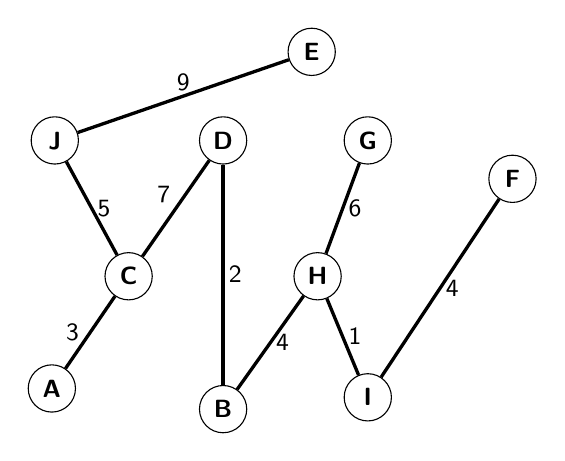
\begin{tikzpicture}[x=0.75cm,y=0.75cm,v/.style={circle,draw,fill=white,inner sep=1pt,minimum size=6mm,font=\small\sffamily\bfseries},
  w/.style={font=\small\sffamily,inner sep=1.5pt}]
\node[v] (E) at (5.4,6.05) {E};
\node[v] (J) at (1.05,4.55) {J};
\node[v] (D) at (3.9,4.55) {D};
\node[v] (G) at (6.35,4.55) {G};
\node[v] (F) at (8.8,3.9) {F};
\node[v] (C) at (2.3,2.25) {C};
\node[v] (H) at (5.5,2.25) {H};
\node[v] (A) at (1.0,0.35) {A};
\node[v] (B) at (3.9,0) {B};
\node[v] (I) at (6.35,0.2) {I};
\draw[very thick] (A)--node[w,left=2pt]{3}(C);
\draw[very thick] (C)--node[w,right]{5}(J);
\draw[very thick] (C)--node[w,above left]{7}(D);
\draw[very thick] (D)--node[w,right]{2}(B);
\draw[very thick] (B)--node[w,right]{4}(H);
\draw[very thick] (H)--node[w,right]{1}(I);
\draw[very thick] (I)--node[w,right]{4}(F);
\draw[very thick] (H)--node[w,right]{6}(G);
\draw[very thick] (J)--node[w,above]{9}(E);
\end{tikzpicture}
\end{center}

(b) 總權重 $3 + 5 + 7 + 2 + 4 + 1 + 4 + 6 + 9 = 41$。 用 Kruskal 從最輕的邊加起，也得到總權重 $41$。
\end{pastsoln}
